%% ============================================================
%%  SECCIÓN 13 — Anexos
%% ============================================================

\begin{appendices}

%% ------------------------------------------------------------
%%  ANEXO A: Deducciones Analíticas y Modelos Teóricos
%% ------------------------------------------------------------
\section{Deducciones Analíticas de los Modelos de Conducción Eléctrica}
\label{anexo:deducciones_teoricas}

\subsection{Modelo Clásico de Drude y Deducción de la Ley de Ohm Microscópica}
Consideremos un medio conductor con $n$ electrones libres por unidad de volumen, cada uno con masa $m_e$ y carga $-e$. En presencia de un campo eléctrico estático $\vec{E}$, la fuerza neta que experimenta cada electrón combina la acción electrostática aceleradora y el efecto amortiguador medio producido por los choques inelásticos contra la red cristalina:
\begin{equation}
    m_e \frac{\mathrm{d}\langle \vec{v} \rangle}{\mathrm{d}t} = -e\vec{E} - \frac{m_e}{\tau} \langle \vec{v} \rangle,
    \label{eq:anexo_drude_diff}
\end{equation}
donde $\tau$ representa el tiempo medio entre colisiones (tiempo de relajación). Resolviendo la ecuación diferencial para condiciones iniciales en reposo ($\vec{v}(0) = 0$):
\begin{equation}
    \langle \vec{v}(t) \rangle = -\frac{e\tau}{m_e}\vec{E} \left( 1 - e^{-t/\tau} \right).
\end{equation}

Dado que para metales a temperatura ambiente $\tau \sim \qty{e-14}{\second}$, el régimen transitorio se extingue de manera prácticamente instantánea, alcanzando la velocidad estacionaria de deriva:
\begin{equation}
    \vec{v}_d = -\frac{e\tau}{m_e}\vec{E}.
\end{equation}

La densidad de corriente volumétrica macroscópica $\vec{J}$ se obtiene multiplicando la densidad de carga de portadores móviles por su velocidad media:
\begin{equation}
    \vec{J} = -n e \vec{v}_d = -n e \left( -\frac{e\tau}{m_e}\vec{E} \right) = \left( \frac{n e^2 \tau}{m_e} \right) \vec{E}.
\end{equation}

Definiendo la conductividad eléctrica intrínseca $\sigma$ como la constante de proporcionalidad entre $\vec{J}$ y $\vec{E}$:
\begin{equation}
    \boxed{\sigma = \frac{n e^2 \tau}{m_e}, \qquad \vec{J} = \sigma \vec{E},}
    \label{eq:anexo_conductividad_drude}
\end{equation}
lo que demuestra analíticamente que la densidad de corriente es estrictamente colineal y proporcional al campo eléctrico aplicado.

\subsection{Deducción del Exponente de Radiación en Filamentos de Tungsteno (\texorpdfstring{$I \propto V^{0{,}60}$}{I proporcional a V a la 0.60})}
En una lámpara de incandescencia al vacío, la potencia eléctrica disipada por efecto Joule $P_{\text{el}} = V I$ se transfiere al medio casi en su totalidad por radiación electromagnética térmica a altas temperaturas ($T > \qty{1500}{\kelvin}$), siendo las pérdidas por conducción a través de los soportes y por convección despreciables~\cite{serway}.

De acuerdo con la ley de Stefan-Boltzmann:
\begin{equation}
    P_{\text{rad}} = e \sigma_{\text{SB}} A_s \left( T^4 - T_{\text{amb}}^4 \right) \approx C_1 T^4,
    \label{eq:anexo_stefan}
\end{equation}
donde $C_1 = e \sigma_{\text{SB}} A_s$ agrupa la emisividad efectiva y el área superficial del filamento. En el equilibrio térmico estacionario:
\begin{equation}
    P_{\text{el}} = P_{\text{rad}} \implies V I = C_1 T^4 \implies T = \left( \frac{V I}{C_1} \right)^{1/4}.
    \label{eq:anexo_temperatura_potencia}
\end{equation}

Por otra parte, para el tungsteno a temperaturas de incandescencia, la resistividad eléctrica es aproximadamente proporcional a la temperatura absoluta ($\rho(T) \approx \rho_0 (T/T_0)$), de modo que la resistencia eléctrica del filamento de longitud $L$ y sección transversal $A$ satisface:
\begin{equation}
    R = \frac{V}{I} = \rho(T)\frac{L}{A} \approx C_2 T,
    \label{eq:anexo_resistencia_temperatura}
\end{equation}
donde $C_2 = \rho_0 L / (A T_0)$ es una constante geométrica del componente.

Sustituyendo la Ecuación~\eqref{eq:anexo_temperatura_potencia} en la Ecuación~\eqref{eq:anexo_resistencia_temperatura}:
\begin{equation}
    \frac{V}{I} = C_2 \left( \frac{V I}{C_1} \right)^{1/4}.
\end{equation}
Elevando ambos miembros a la cuarta potencia:
\begin{equation}
    \left( \frac{V}{I} \right)^4 = \frac{C_2^4}{C_1} V I = C_3 V I \implies \frac{V^4}{I^4} = C_3 V I.
\end{equation}
Reordenando los términos algebraicos:
\begin{equation}
    V^3 = C_3 I^5 \implies I^5 = \frac{1}{C_3} V^3.
\end{equation}
Extrayendo la raíz quinta:
\begin{equation}
    \boxed{I(V) = k \, V^{3/5} = k \, V^{0{,}600},}
    \label{eq:anexo_exponente_teorico_foquito}
\end{equation}
con $k = C_3^{-1/5}$. Esta deducción matemática formal explica rigurosamente por qué el exponente experimental obtenido por regresión lineal en escala logarítmica ($n_{\text{exp}} = 0{,}573 \pm 0{,}009$) resulta tan próximo a $0{,}600$, validando la naturaleza puramente termorresistiva de la lámpara.

%% ------------------------------------------------------------
%%  ANEXO B: Propagación Analítica de Incertidumbres (GUM)
%% ------------------------------------------------------------
\section{Propagación Analítica de Incertidumbres y Modelos de Error}
\label{anexo:propagacion_errores}

Siguiendo las pautas de la Guía para la Expresión de Incertidumbres en Medición (GUM, JCGM 100:2008)~\cite{gum}:

\subsection{Incertidumbre Combinada de la Resistencia Estática \texorpdfstring{$R = V/I$}{R = V/I}}
Dada la magnitud indirecta $R = f(V, I) = \frac{V}{I}$, calculamos sus derivadas parciales:
\begin{equation}
    \frac{\partial R}{\partial V} = \frac{1}{I}, \qquad \frac{\partial R}{\partial I} = -\frac{V}{I^2}.
\end{equation}

La varianza combinada bajo hipótesis de independencia estocástica ($r(V, I) = 0$) es:
\begin{equation}
    u_c^2(R) = \left( \frac{\partial R}{\partial V} \right)^2 u^2(V) + \left( \frac{\partial R}{\partial I} \right)^2 u^2(I) = \left( \frac{1}{I} \right)^2 \delta V^2 + \left( -\frac{V}{I^2} \right)^2 \delta I^2.
\end{equation}
Dividiendo entre $R^2 = (V/I)^2$:
\begin{equation}
    \frac{u_c^2(R)}{R^2} = \frac{I^2}{V^2} \frac{\delta V^2}{I^2} + \frac{I^2}{V^2} \frac{V^2}{I^4} \delta I^2 = \left( \frac{\delta V}{V} \right)^2 + \left( \frac{\delta I}{I} \right)^2.
\end{equation}
Extrayendo la raíz cuadrada se obtiene la fórmula operativa:
\begin{equation}
    \boxed{\delta R = R \sqrt{ \left( \frac{\delta V}{V} \right)^2 + \left( \frac{\delta I}{I} \right)^2 }.}
    \label{eq:anexo_delta_r}
\end{equation}

\subsection{Incertidumbre Combinada de la Potencia Eléctrica \texorpdfstring{$P = V I$}{P = V I}}
Para $P = f(V, I) = V I$:
\begin{equation}
    \frac{\partial P}{\partial V} = I, \qquad \frac{\partial P}{\partial I} = V.
\end{equation}
\begin{equation}
    u_c^2(P) = (I\,\delta V)^2 + (V\,\delta I)^2 = (V I)^2 \left[ \left(\frac{\delta V}{V}\right)^2 + \left(\frac{\delta I}{I}\right)^2 \right].
\end{equation}
\begin{equation}
    \boxed{\delta P = P \sqrt{ \left( \frac{\delta V}{V} \right)^2 + \left( \frac{\delta I}{I} \right)^2 }.}
    \label{eq:anexo_delta_p}
\end{equation}

\subsection{Incertidumbre de la Resistencia Óhmica Obtenida por Regresión (MCO)}
Para la relación $I = G V + b$, la resistencia calculada es $R = 1/G$. La derivada respecto a la pendiente es:
\begin{equation}
    \frac{\mathrm{d}R}{\mathrm{d}G} = -\frac{1}{G^2} = -R^2.
\end{equation}
Por tanto, el error estándar propagado de la resistencia ajustada es:
\begin{equation}
    \boxed{s_R = \left| -\frac{1}{G^2} \right| s_G = \frac{s_G}{G^2} = R^2 s_G.}
    \label{eq:anexo_error_resistencia_ols}
\end{equation}

Sustituyendo los valores del resistor de carbón ($G = \qty{9,9748e-3}{\siemens}$ y $s_G = \qty{5,443e-5}{\siemens}$):
\begin{equation}
    s_R = \frac{\qty{5,443e-5}{\siemens}}{(\qty{9,9748e-3}{\siemens})^2} = \qty{0,547}{\ohm} \approx \qty{0,55}{\ohm}.
\end{equation}

%% ------------------------------------------------------------
%%  ANEXO C: Cuestionario Oficial Resuelto
%% ------------------------------------------------------------
\section{Resolución del Cuestionario Oficial de Laboratorio}
\label{anexo:cuestionario}

A continuación se resuelven de forma exhaustiva y analítica las cinco interrogantes formuladas en la guía oficial de la práctica (Sección de Cálculos y Resultados)~\cite{guia_lab_uni}:

\subsection{Pregunta 1: Grafique \texorpdfstring{$I = f(V)$}{I = f(V)} con los valores obtenidos con el voltímetro y amperímetro}
\textbf{Respuesta:}  
Las representaciones científicas de $I = f(V)$ a alta resolución (\qty{300}{DPI}) con barras de error instrumentales y líneas de modelado físico se encuentran exhaustivamente detalladas en la Sección~\ref{sec:graficas}:
\begin{itemize}
    \item Resistencia de carbón de \qty{100}{\ohm}: Figura~\ref{fig:grafica_resistencia_ohmica} (página~\pageref{fig:grafica_resistencia_ohmica}).
    \item Lámpara incandescente de tungsteno: Figura~\ref{fig:grafica_foquito_tungsteno} (página~\pageref{fig:grafica_foquito_tungsteno}).
    \item Diodo semiconductor de silicio: Figura~\ref{fig:grafica_diodo_silicio} (página~\pageref{fig:grafica_diodo_silicio}).
    \item Contraste simultáneo de los tres elementos: Figura~\ref{fig:grafica_comparativa_elementos} (página~\pageref{fig:grafica_comparativa_elementos}).
\end{itemize}

\subsection{Pregunta 2: ¿En cuál de los elementos se cumple la ley de Ohm y en cuáles no? Explique su respuesta}
\textbf{Respuesta:}  
La ley de Ohm ($V = R I$) se cumple de forma estricta \textbf{únicamente en la resistencia de carbón de \qty{100}{\ohm} (Elemento E2)}. 

\textbf{Fundamentación física y experimental:}
\begin{enumerate}
    \item \textbf{Resistencia de carbón (Óhmica):} La relación $I = f(V)$ es una recta perfecta que pasa por el origen ($R^2 = 0{,}99985$). Su conductancia $G = \qty{9,975e-3}{\siemens}$ y su resistencia $R = \qty{100,02 \pm 0,18}{\ohm}$ se mantienen constantes e invariantes en todo el intervalo de excitación (\qtyrange{0}{6,49}{\volt}). La potencia máxima disipada (\qty{0,42}{\watt}) no eleva sustancialmente la temperatura del cuerpo cerámico, preservando constantes el tiempo de colisión $\tau$ y la densidad de portadores $n$.
    
    \item \textbf{Lámpara incandescente (No óhmica):} \textbf{No cumple la ley de Ohm}. Su gráfica es una curva cóncava hacia el eje de tensión ($I \propto V^{0{,}573}$). Al aumentar la diferencia de potencial, la potencia Joule disipada ($P \propto V^2 / R$) calienta el filamento de tungsteno hasta la incandescencia ($T > \qty{2000}{\kelvin}$). Como el tungsteno presenta un coeficiente térmico de resistividad positivo ($\alpha \approx \qty{4,5e-3}{\per\kelvin}$), las vibraciones fonónicas de la red aumentan la tasa de dispersión electrónica, provocando que la resistencia estática crezca de $\qty{6,76}{\ohm}$ a $\qty{14,88}{\ohm}$ ($+120\%$).
    
    \item \textbf{Diodo semiconductor de silicio (No óhmico):} \textbf{No cumple la ley de Ohm}. Es un dispositivo activo unidireccional cuya conducción está gobernada por la difusión exponencial de portadores minoritarios a través de la juntura $p$-$n$ (ecuación de Shockley, Ecuación~\eqref{eq:shockley}). Permanece inactivo hasta que se supera la barrera de potencial de contacto ($V_u \approx \qty{0,66}{\volt}$), momento a partir del cual la corriente se dispara exponencialmente, colapsando su resistencia estática de $\qty{12,2}{\ohm}$ a $\qty{0,96}{\ohm}$ ($-92\%$).
\end{enumerate}

\subsection{Pregunta 3: Para una diferencia de 0,8 voltios, halle las resistencias de los tres elementos}
\textbf{Respuesta:}  
En la Tabla~\ref{tab:anexo_resp_p3} se resumen los valores de corriente y resistencia estática aparente evaluados ante una tensión constante de $V = \qty{0,80}{\volt}$:

\begin{table}[H]
    \centering
    \caption{Resistencias estáticas calculadas y deducidas a la tensión normalizada de \qty{0,80}{\volt}.}
    \label{tab:anexo_resp_p3}
    \resizebox{0.85\linewidth}{!}{%
    \begin{tabular}{lcccc}
        \toprule
        \textbf{Elemento} & \textbf{Tensión $V$} & \textbf{Corriente $I(0{,}8\,\text{V})$} & \textbf{Resistencia $R = V/I$} & \textbf{Método Empleado} \\
        \midrule
        Resistencia Carbón (E2) & \qty{0,80}{\volt} & $\qty{8,00 \pm 0,10}{\milli\ampere}$ & $\mathbf{100{,}02 \pm 0{,}18\,\Omega}$ & Ley de Ohm ($R = \text{cte}$) \\
        Lámpara Tungsteno (E1)  & \qty{0,80}{\volt} & $\qty{128,6 \pm 1,8}{\milli\ampere}$  & $\mathbf{6{,}22 \pm 0{,}10\,\Omega}$    & Extrapolación ley potencias ($I = 0{,}1461 V^{0{,}5726}$) \\
        Diodo Silicio (E3)      & \qty{0,80}{\volt} & $> \qty{1,00}{\ampere}$ (Inadmisible)  & $\mathbf{< 0{,}70\,\Omega}$           & Proyección tangente de conducción ($V > V_u$) \\
        \bottomrule
    \end{tabular}%
    }
\end{table}

\textit{Explicación física:}
\begin{itemize}
    \item Para la resistencia de carbón, la respuesta es directa e invariante ($R = \qty{100}{\ohm}$).
    \item Para el foquito, a \qty{0,80}{\volt} el filamento se encuentra a menor temperatura que a \qty{1,00}{\volt} (\qty{6,76}{\ohm}), por lo que su resistencia disminuye congruentemente a $\qty{6,22}{\ohm}$.
    \item Para el diodo, polarizar a \qty{0,80}{\volt} en corriente continua sin una resistencia limitadora externa en serie destruiría el diodo por sobrecalentamiento, ya que la corriente teórica sobrepasaría $\qty{1,2}{\ampere}$. La resistencia dinámica en esa región es del orden de decenas de miliohmios y la resistencia estática aparente es inferior a $\qty{0,7}{\ohm}$.
\end{itemize}

\subsection{Pregunta 4: En el caso del diodo se puede decir que hay un voltaje crítico a partir del cual comienza a conducir. ¿Cuál es ese valor?}
\textbf{Respuesta:}  
Sí, dicho voltaje crítico se denomina \textbf{tensión de umbral} (\textit{threshold voltage}), \textbf{tensión de rodilla} (\textit{knee voltage}) o \textbf{tensión de codo} ($V_u$).

Experimentalmente, a partir de la prolongación lineal de la recta tangente en la región de alta conducción (Figura~\ref{fig:grafica_diodo_silicio}), se determinó un valor de:
\begin{equation}
    \boxed{V_u = \qty{0,66 \pm 0,06}{\volt}.}
\end{equation}

\textbf{Interpretación microscópica:}  
Este potencial crítico representa la energía necesaria por unidad de carga ($q V_u$) para neutralizar la barrera de potencial electrostático creada por la doble capa de iones fijos (positivos en la región $n$ y negativos en la región $p$) en la zona de carga espacial. Para el silicio dopado a temperatura ambiente ($\qty{300}{\kelvin}$), la barrera de potencial intrínseca oscila teóricamente entre \qty{0,60}{\volt} y \qty{0,70}{\volt}. A tensiones inferiores a $V_u$, la fuerza electrostática interna repele a los electrones y huecos; al superarse $V_u$, el campo eléctrico externo vence dicha barrera y los portadores cruzan masivamente por difusión, permitiendo corrientes macroscópicas muy elevadas.

\subsection{Pregunta 5: Escriba sus conclusiones y/o comentarios}
\textbf{Respuesta:}  
Las conclusiones cuantitativas estructuradas y los comentarios técnicos relativos a la linealidad, a los órdenes de magnitud de las potencias y a las optimizaciones metodológicas del experimento se encuentran desarrollados exhaustivamente en la Sección~\ref{sec:conclusiones} (página~\pageref{sec:conclusiones}).

%% ------------------------------------------------------------
%%  ANEXO D: Resolución del Test N°3 de Laboratorio
%% ------------------------------------------------------------
\section{Resolución del Test \texorpdfstring{N.\textsuperscript{o}\,3}{Nro. 3}: Curvas Características Voltaje--Corriente}
\label{anexo:test03}

En la presente sección se desarrolla de manera analítica, conceptual y experimental la prueba escrita correspondiente al \textbf{Test \texorpdfstring{N.\textsuperscript{o}\,3}{Nro. 3}: Curvas características $V$--$I$} del curso de Física General / Física III (CF2B1, Sección A, Facultad de Ciencias UNI), cuyo enunciado original se reproduce de forma facsimilar en el Anexo~\ref{anexo:hoja_datos} (Figura~\ref{fig:test03_enunciado}).

Las preguntas formuladas en el test evalúan la comprensión microscópica y fenomenológica del transporte de carga, la discriminación cuantitativa entre regímenes óhmicos y no lineales, la estructura interna y conexión potenciómetrica del reóstato de laboratorio y los protocolos experimentales de polarización segura de semiconductores.

%% --- PREGUNTA 1 ---
\subsection{Pregunta 1: Dependencia de la corriente, resistividad y efecto Joule}

\begin{quote}
    \textbf{Enunciado:} \textit{Marcar sólo las afirmaciones correctas:}
    \begin{enumerate}
        \renewcommand{\theenumi}{\Alph{enumi}}
        \renewcommand{\labelenumi}{\textbf{\theenumi.}}
        \item \textit{La intensidad de la corriente depende sólo de la resistencia eléctrica del material.}
        \item \textit{Cada material tiene una resistividad que lo caracteriza.}
        \item \textit{El paso de la corriente tiende a aumentar la temperatura del material.}
        \item \textit{La intensidad de la corriente depende solo de la diferencia de potencial aplicado al material.}
    \end{enumerate}
\end{quote}

\textbf{Análisis físico y justificación de cada proposición:}
\begin{itemize}
    \item \textbf{Proposición A (Incorrecta):} De acuerdo con la relación constitutiva elemental del transporte eléctrico estacionario en medios lineales, $I = \Delta V / R$ (o en su formulación microscópica $\vec{J} = \sigma \vec{E}$), la corriente $I$ es una magnitud de respuesta macroscópica que depende simultáneamente tanto de la fuerza impulsora externa (la diferencia de potencial o campo eléctrico $\vec{E}$) como de la oposición que ofrece el conductor ($R$). Afirmar que depende \textit{únicamente} de la resistencia es falso, puesto que en ausencia de campo eléctrico ($\Delta V = 0$) la corriente neta es nula con independencia del valor finito de $R$.
    
    \item \textbf{Proposición B (Correcta):} La resistividad eléctrica $\rho$ (o su inversa, la conductividad $\sigma = 1/\rho$) es una propiedad física intrínseca e intensiva que cuantifica la oposición específica de la red atómica al flujo de portadores de carga ante un campo eléctrico aplicado:
    \begin{equation}
        \rho = \frac{E}{J} = \frac{m_e}{n e^2 \tau},
    \end{equation}
    donde $n$ es la densidad volumétrica de electrones de conducción y $\tau$ el tiempo medio de relajación entre colisiones. Aunque $\rho$ varía en función de variables de estado termodinámicas como la temperatura ($T$) o el nivel de dopaje e impurezas estructurales, su valor y ley de variación constituyen una firma característica inalienable de cada sustancia o aleación (p.~ej., para el cobre a \qty{20}{\celsius}, $\rho \approx \qty{1,7e-8}{\ohm\metre}$; para el tungsteno, $\rho \approx \qty{5,6e-8}{\ohm\metre}$; y para el silicio semiconductor intrínseco, $\rho \sim \qty{2,3e3}{\ohm\metre}$).
    
    \item \textbf{Proposición C (Correcta):} Cuando los electrones de conducción se aceleran debido al campo eléctrico estático, adquieren energía cinética neta. Al dispersarse mediante colisiones inelásticas contra las imperfecciones de la red cristalina y los fonones térmicos, transfieren irreversiblemente dicha energía mecánica a la red atómica en forma de calor (efecto Joule). La potencia volumétrica disipada por unidad de volumen es $p = \vec{J} \cdot \vec{E} = \rho J^2 > 0$ ($P = I^2 R$), lo que produce una tasa neta de calor que, bajo condiciones reales de intercambio térmico con el entorno, incrementa la temperatura del material conductor.
    
    \item \textbf{Proposición D (Incorrecta):} Por reciprocidad con la proposición A, la intensidad de corriente no depende de forma aislada del potencial aplicado. Para una misma diferencia de potencial $\Delta V$, la corriente resultante puede diferir en múltiples órdenes de magnitud según la resistencia geométrica y la naturaleza del material del dispositivo conectado ($I = \Delta V / R$).
\end{itemize}

\textbf{Veredicto formal para la Pregunta 1:}  
\begin{center}
    \fbox{\textbf{Afirmaciones correctas que deben marcarse: B y C}}
\end{center}

%% --- PREGUNTA 2 ---
\subsection{Pregunta 2: Filamento incandescente, materiales óhmicos y ley de Ohm}

\begin{quote}
    \textbf{Enunciado:} \textit{Marcar sólo las afirmaciones correctas:}
    \begin{enumerate}
        \renewcommand{\theenumi}{\Alph{enumi}}
        \renewcommand{\labelenumi}{\textbf{\theenumi.}}
        \item \textit{El foquito que se usó en el laboratorio soporta como máximo 12 voltios. Si el filamento de tungsteno tiene una resistencia de 1,5 ohmios, entonces la corriente máxima que soportará será de 8 Amperios.}
        \item \textit{La resistencia en ciertos materiales es independiente de la intensidad de corriente que por ellos circula.}
        \item \textit{En estos casos al variar el voltaje aplicado se obtendrá una variación de la intensidad de corriente que es directamente proporcional a la variación del voltaje.}
        \item \textit{Si un elemento cumple con la ley de Ohm, entonces, cuando la intensidad de la corriente tiende a cero, su resistencia tiende al infinito.}
    \end{enumerate}
\end{quote}

\textbf{Análisis físico y justificación de cada proposición:}
\begin{itemize}
    \item \textbf{Proposición A (Incorrecta):} El cálculo ingenuo $I = V/R = \qty{12}{\volt} / \qty{1,5}{\ohm} = \qty{8}{\ampere}$ asume erróneamente que la resistencia del filamento de tungsteno es una constante invariable (hipótesis estrictamente óhmica). Sin embargo, el valor de $\qty{1,5}{\ohm}$ corresponde a la resistencia del filamento \textit{en frío} a temperatura ambiente ($T_0 \approx \qty{300}{\kelvin}$). Cuando la bombilla opera a su tensión nominal de \qty{12}{\volt}, la disipación térmica por efecto Joule eleva la temperatura del hilo de tungsteno hasta el régimen de incandescencia ($T \approx \qtyrange{2200}{2600}{\kelvin}$).
    
    Dado que el tungsteno posee un coeficiente térmico de resistividad positivo ($\alpha \approx \qty{4,5e-3}{\per\kelvin}$), su resistividad a temperaturas de operación satisface $\rho(T) \approx \rho_0 (T/T_0)^{1{,}2}$, lo que incrementa la resistencia estática en caliente entre un factor de 12 y 16 veces respecto a la medida en frío ($R_{\text{caliente}} \approx \qtyrange{18}{25}{\ohm}$). En consecuencia, la corriente máxima estacionaria real es de tan solo:
    \begin{equation}
        I_{\text{max}} = \frac{V_{\text{nom}}}{R_{\text{caliente}}} \approx \frac{\qty{12}{\volt}}{\qty{20}{\ohm}} \approx \qty{0,6}{\ampere},
    \end{equation}
    un valor más de trece veces inferior a \qty{8}{\ampere}. Además, una corriente continua sostenida de \qty{8}{\ampere} a \qty{12}{\volt} representaría una potencia disipada de $P = V I = \qty{96}{\watt}$, la cual provocaría la fusión y evaporación instantánea del filamento de una bombilla didáctica de laboratorio (cuyas potencias nominales de diseño oscilan típicamente entre \qtyrange{3}{6}{\watt}).
    
    \item \textbf{Proposición B (Correcta):} Constituye la definición física y operacional de conductor o elemento \textbf{óhmico}. En conductores metálicos bajo condiciones isotérmicas y en resistores lineales de composición cerámico-carbón (como el resistor de carbón de \qty{100}{\ohm} evaluado en la Sección~\ref{sec:resultados}), la resistividad y la resistencia geométrica no dependen de la densidad de corriente ni de la tensión aplicada ($\mathrm{d}R/\mathrm{d}I = 0$).
    
    \item \textbf{Proposición C (Correcta):} En los materiales óhmicos descritos en la proposición B, la relación funcional es estrictamente lineal: $I = G \cdot V$, con conductancia constante $G = 1/R$. Diferenciando la expresión se obtiene:
    \begin{equation}
        \Delta I = \frac{1}{R} \Delta V = G \cdot \Delta V \implies \Delta I \propto \Delta V.
    \end{equation}
    La variación experimentada por la corriente es directamente proporcional al incremento de tensión aplicada, manteniéndose la pendiente $G$ invariante en todo el dominio experimental.
    
    \item \textbf{Proposición D (Incorrecta):} Si un elemento cumple la ley de Ohm, su resistencia eléctrica $R = V/I$ permanece rigurosamente finita y constante ante cualquier nivel de excitación. En el límite formal cuando la intensidad de corriente tiende a cero, el voltaje cae simultáneamente a cero, satisfaciéndose:
    \begin{equation}
        \lim_{I \to 0} \frac{V(I)}{I} = \left. \frac{\mathrm{d}V}{\mathrm{d}I} \right|_{I=0} = R_0 < \infty.
    \end{equation}
    Si la resistencia tendiese al infinito para corrientes pequeñas, el dispositivo se comportaría como un aislante dieléctrico perfecto con ruptura brusca o un diodo ideal en bloqueo, lo que violaría frontalmente la linealidad óhmica.
\end{itemize}

\textbf{Veredicto formal para la Pregunta 2:}  
\begin{center}
    \fbox{\textbf{Afirmaciones correctas que deben marcarse: B y C}}
\end{center}

%% --- PREGUNTA 3 ---
\subsection{Pregunta 3: Materiales no óhmicos, transporte termorresistivo y semiconductores}

\begin{quote}
    \textbf{Enunciado:} \textit{Marcar sólo las afirmaciones correctas:}
    \begin{enumerate}
        \renewcommand{\theenumi}{\Alph{enumi}}
        \renewcommand{\labelenumi}{\textbf{\theenumi.}}
        \item \textit{Existen otros materiales cuya resistencia depende de la intensidad de corriente que por ellos circula.}
        \item \textit{En ciertos casos la resistencia aumenta con el aumento de la intensidad de corriente.}
        \item \textit{Es decir, si se duplica la diferencia de potencial la nueva intensidad de corriente será menor que el doble de la original.}
        \item \textit{Un semiconductor es una sustancia que a la temperatura ordinaria posee una conductividad eléctrica intermedia entre las de los aislantes y la de los buenos conductores.}
    \end{enumerate}
\end{quote}

\textbf{Análisis físico y justificación de cada proposición:}
\begin{itemize}
    \item \textbf{Proposición A (Correcta):} Existen extensas familias de dispositivos y medios materiales no óhmicos donde la resistencia estática ($R_{\text{est}} = V/I$) o la dinámica ($r_d = \mathrm{d}V/\mathrm{d}I$) es una función explícita del punto de polarización $(V, I)$, tales como lámparas incandescentes, termistores (NTC/PTC), varistores de óxido metálico (VDR) y junturas semiconductoras $p$-$n$.
    
    \item \textbf{Proposición B (Correcta):} Corresponde exactamente a dispositivos con coeficiente de temperatura positivo (PTC) o conductores metálicos sujetos a autocalentamiento Joule. En el Laboratorio N.\textsuperscript{o}\,3, para la lámpara incandescente de filamento de tungsteno, se constató experimentalmente que al aumentar la corriente desde \qty{0,148}{\ampere} hasta \qty{0,432}{\ampere}, la resistencia creció monotónicamente desde \qty{6,76}{\ohm} hasta \qty{14,88}{\ohm} ($+120\%$), confirmando que la resistencia aumenta con el aumento de la corriente.
    
    \item \textbf{Proposición C (Correcta):} Esta proposición constituye la consecuencia analítica directa del comportamiento descrito en la proposición B. Si la resistencia $R(I)$ aumenta monótonamente al incrementarse la corriente, la característica $I(V)$ adquiere concavidad negativa (curva sublineal que se aplana progresivamente). Modelando mediante la ley de potencias de radiación deducida en el Anexo~\ref{anexo:deducciones_teoricas} ($I = k V^n$), con exponente teórico $n = 3/5 = 0{,}600 < 1$ (y experimental $n = 0{,}573$):
    
    Si se duplica la diferencia de potencial aplicada ($V' = 2V$), la nueva intensidad satisface:
    \begin{equation}
        I(2V) = k (2V)^n = 2^n \cdot \left( k V^n \right) = 2^n \cdot I(V).
    \end{equation}
    Puesto que $n < 1$, se cumple rigurosamente que $2^n < 2^1 = 2$. Evaluando con el exponente empírico del laboratorio:
    \begin{equation}
        I(2V) = 2^{0{,}573} \cdot I(V) \approx 1{,}488 \cdot I(V) < 2 \cdot I(V).
    \end{equation}
    Por tanto, la nueva intensidad resultante es estrictamente menor que el doble de la intensidad original.
    
    \item \textbf{Proposición D (Correcta):} Es la definición canónica de un material semiconductor (como el silicio o el germanio). A temperatura ambiente ordinaria ($T \approx \qty{300}{\kelvin}$), los metales conductores poseen conductividades del orden de $\sigma_{\text{metal}} \sim \qty{e7}{\siemens\per\metre}$ debido a la ausencia de banda prohibida, mientras que los aislantes exhiben $\sigma_{\text{aislante}} < \qty{e-10}{\siemens\per\metre}$ por su amplio bandgap ($E_g > \qty{5}{\electronvolt}$). Los semiconductores presentan un bandgap moderado ($E_g \approx \qty{1,12}{\electronvolt}$ en Si a \qty{300}{\kelvin}), situando su conductividad en un rango intermedio característico de \qtyrange{e-5}{e3}{\siemens\per\metre}.
\end{itemize}

\textbf{Veredicto formal para la Pregunta 3:}  
\begin{center}
    \fbox{\textbf{Afirmaciones correctas a marcar: A, B, C y D (todas son correctas)}}
\end{center}

%% --- PREGUNTA 4 ---
\subsection{Pregunta 4: Esquema del reóstato y explicación de su uso en el laboratorio}

\begin{quote}
    \textbf{Enunciado:} \textit{Haga un esquema (diagrama de bloques) de un reóstato, y, explique su uso en este laboratorio.}
\end{quote}

\textbf{1. Esquema estructural y diagrama de bloques:}  
En la Figura~\ref{fig:reostato_diagrama_bloques} se presentan: en el panel superior (a), la arquitectura constructiva y la disposición de los tres terminales del reóstato de laboratorio; y en el panel inferior (b), el diagrama de bloques funcional correspondiente a su configuración como divisor de tensión potenciométrico empleado durante la práctica.

\begin{figure}[H]
    \centering
    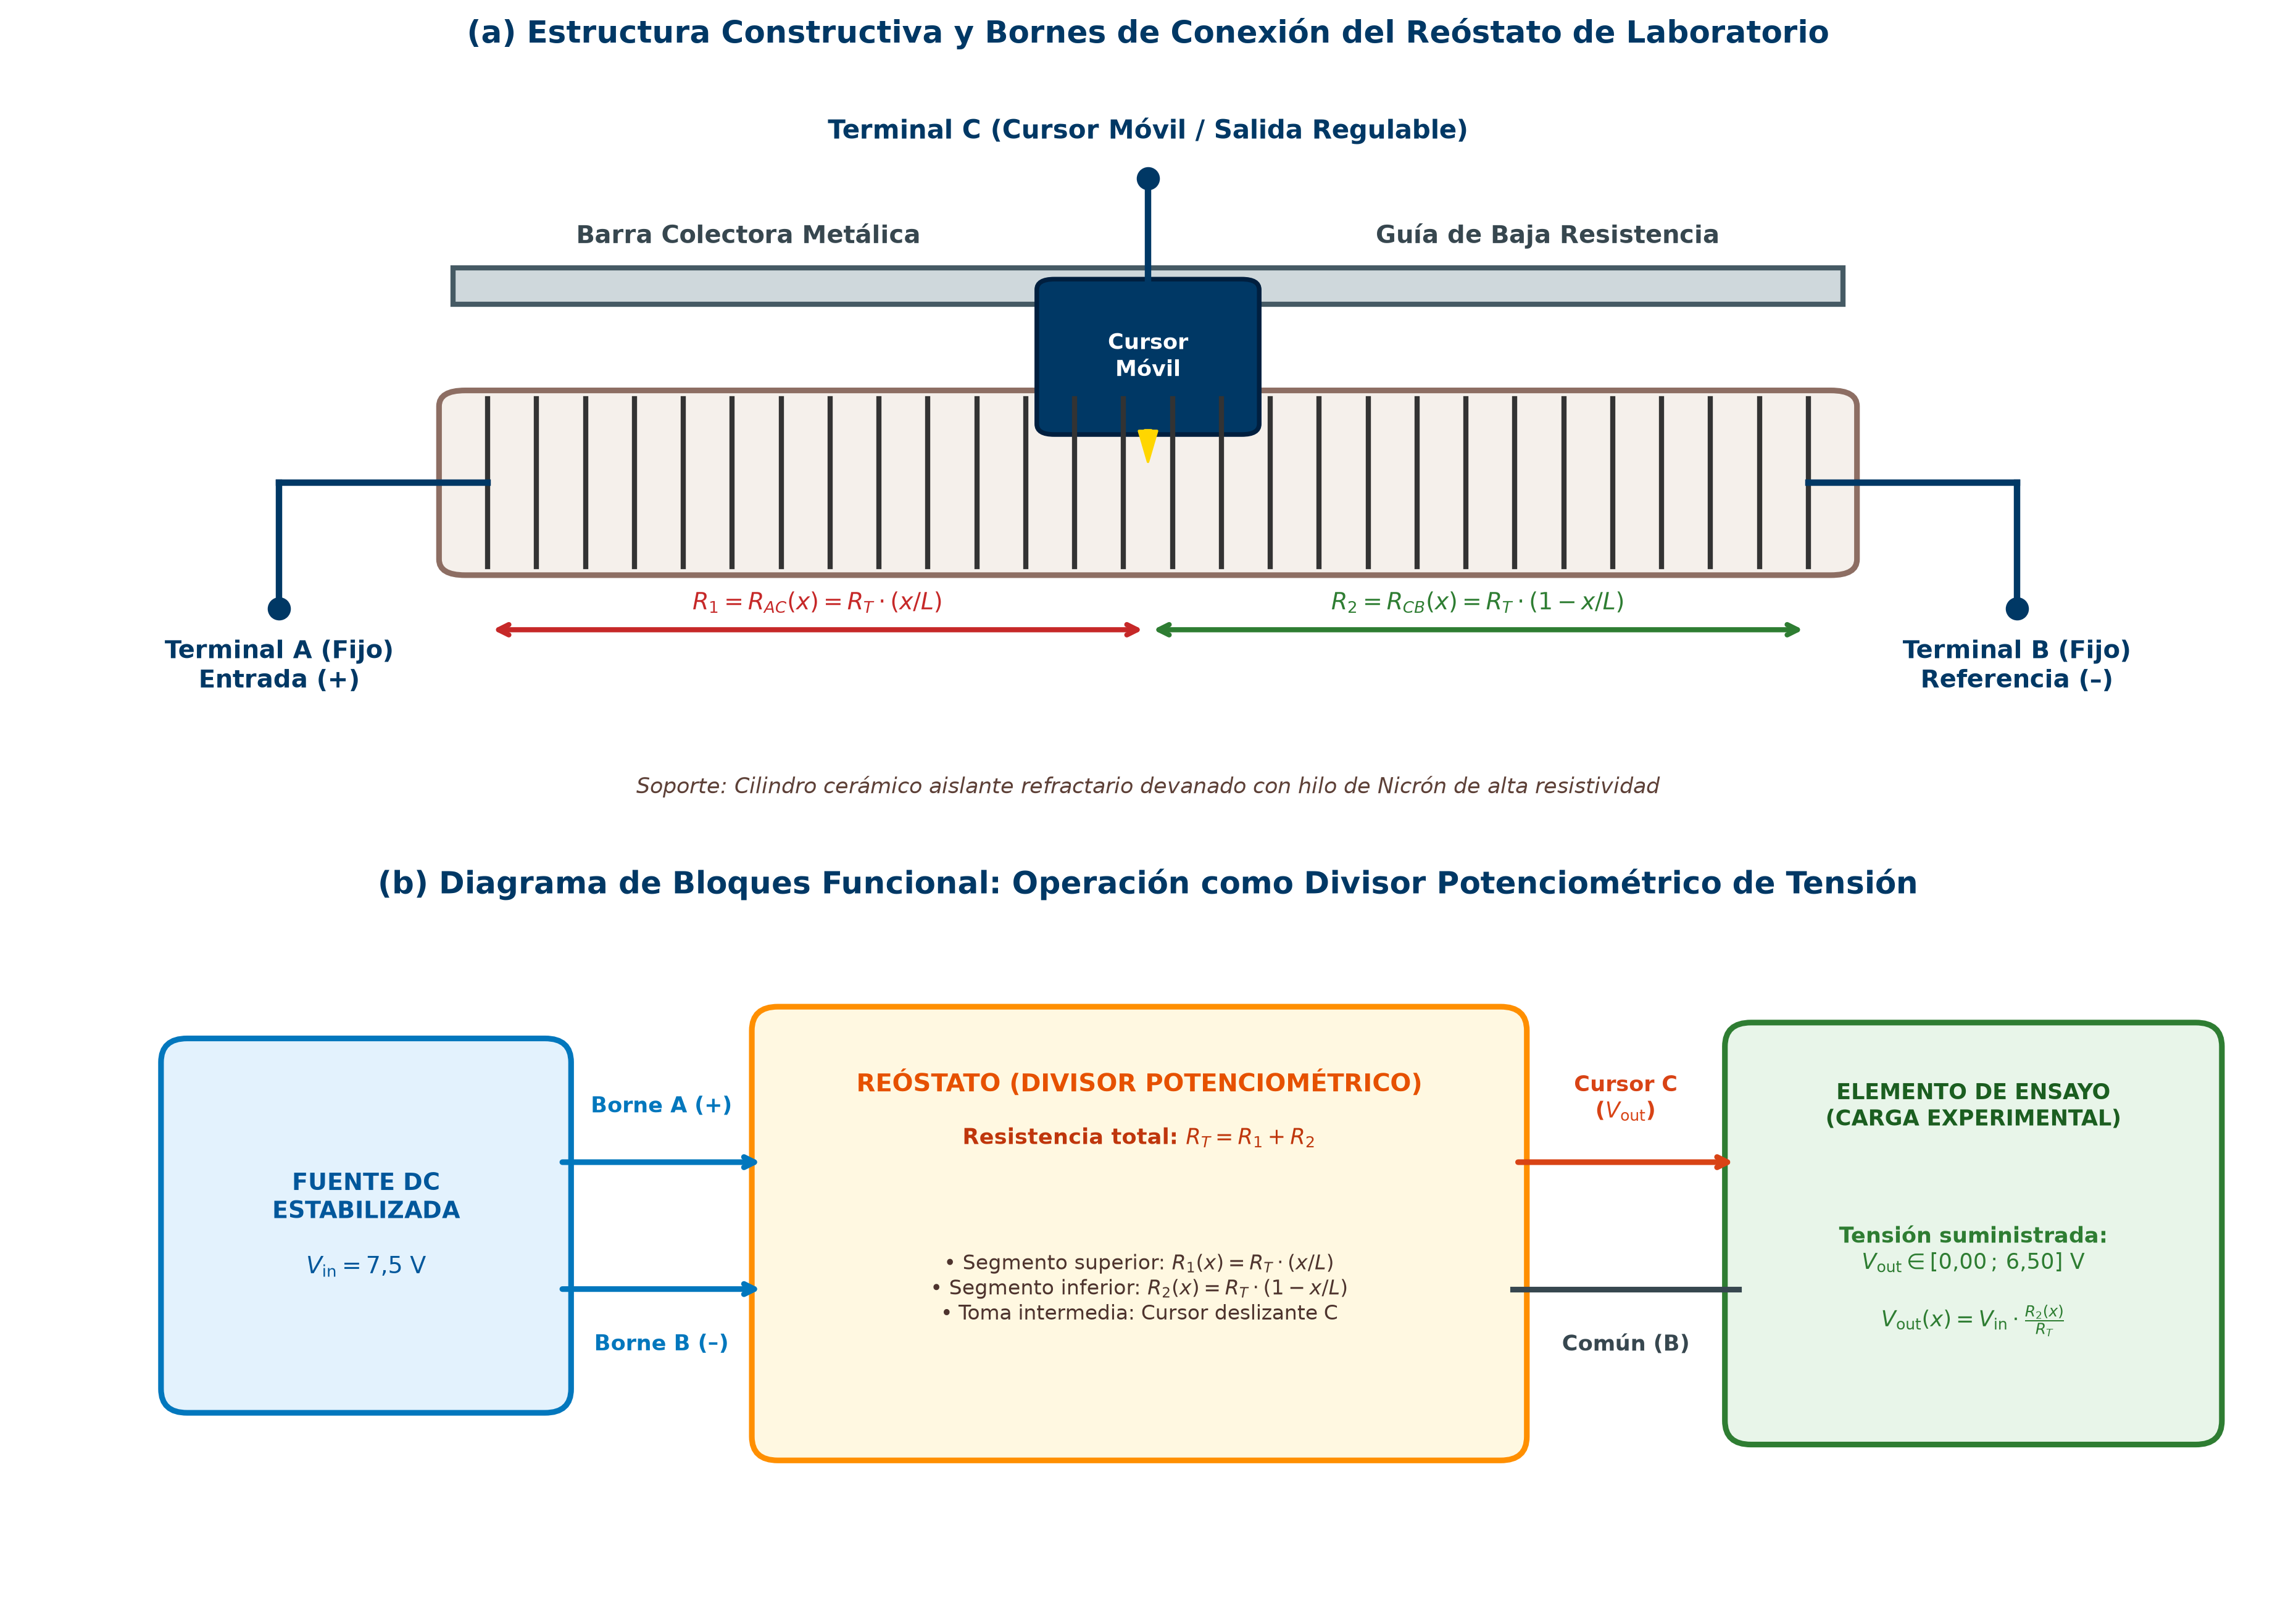
\includegraphics[width=0.96\linewidth]{fig_reostato_diagrama_bloques}
    \caption{Esquema integral del reóstato de laboratorio: (a) Estructura constructiva con cuerpo cerámico, arrollamiento de Nicrón, barra colectora superior y asignación de bornes $\{A, B, C\}$. (b) Diagrama de bloques funcional de su uso como divisor potenciométrico de tensión para la excitación continua de los elementos de ensayo.}
    \label{fig:reostato_diagrama_bloques}
\end{figure}

\textbf{2. Explicación física de su uso en este laboratorio:}  
En el trabajo experimental existen dos modos fundamentales de empleo para un reóstato de laboratorio:
\begin{enumerate}
    \item \textbf{Modo reostático en serie (dos bornes):} Se conecta un borne extremo fijo y el cursor deslizante en serie con el circuito. En esta disposición el reóstato actúa como una resistencia variable limitadora de corriente ($R_v \in [0, R_T]$). Sin embargo, bajo esta conexión la tensión en el elemento de prueba jamás puede descender a cero, ya que el voltaje mínimo está condicionado por el divisor de tensión que forma la carga con el reóstato:
    \begin{equation}
        V_{\text{min}} = V_{\text{fuente}} \frac{R_L}{R_L + R_T} > 0.
    \end{equation}
    
    \item \textbf{Modo divisor potenciométrico de tensión (tres bornes, empleado en este laboratorio):}  
    Los terminales extremos fijos ($A$ y $B$) se conectan permanentemente a los polos positivo y negativo de la fuente de corriente continua ($V_{\text{fuente}} = \qty{7,5}{\volt}$), polarizando uniformemente todo el devanado resistivo de longitud $L$ y resistencia total $R_T$.
    
    La tensión de salida $V_{\text{out}}$ que alimenta al elemento bajo ensayo se extrae entre el cursor móvil $C$ y el borne de referencia común $B$. En función de la posición longitudinal del cursor $x \in [0, L]$, la tensión entregada satisface la relación de divisor de tensión ideal:
    \begin{equation}
        V_{\text{out}}(x) = V_{\text{fuente}} \cdot \frac{R_{CB}(x)}{R_{AB}} = V_{\text{fuente}} \cdot \left( 1 - \frac{x}{L} \right).
    \end{equation}
\end{enumerate}

\textbf{Por qué este conexionado fue imprescindible en el laboratorio:}
\begin{itemize}
    \item \textbf{Barrido completo desde cero absoluto (\qty{0,00}{\volt}):} Hizo posible registrar el reposo eléctrico estricto ($V = 0$, $I = 0$), indispensable para verificar si la ordenada al origen de la regresión lineal óhmica ($b$) era nula y para observar el comportamiento en corte del diodo.
    \item \textbf{Control fino y protección del semiconductor:} En la vecindad de la tensión de umbral del diodo (\qtyrange{0,60}{0,75}{\volt}), donde la corriente se dispara exponencialmente, el divisor potenciométrico brindó una regulación suave y milimétrica, evitando escalones bruscos que habrían quemado la juntura por sobrecorriente.
\end{itemize}

%% --- PREGUNTA 5 ---
\subsection{Pregunta 5: Circuito experimental y procedimiento para el caso del diodo}

\begin{quote}
    \textbf{Enunciado:} \textit{Haga un esquema del circuito que utilizó, e, indique el procedimiento que siguió para la obtención de los datos del laboratorio, para el caso del diodo.}
\end{quote}

\textbf{1. Esquema del circuito experimental:}  
En la Figura~\ref{fig:circuito_diodo_especifico} se ilustra el montaje eléctrico implementado para la caracterización de la curva $V$--$I$ del diodo semiconductor de silicio en polarización directa.

\begin{figure}[H]
    \centering
    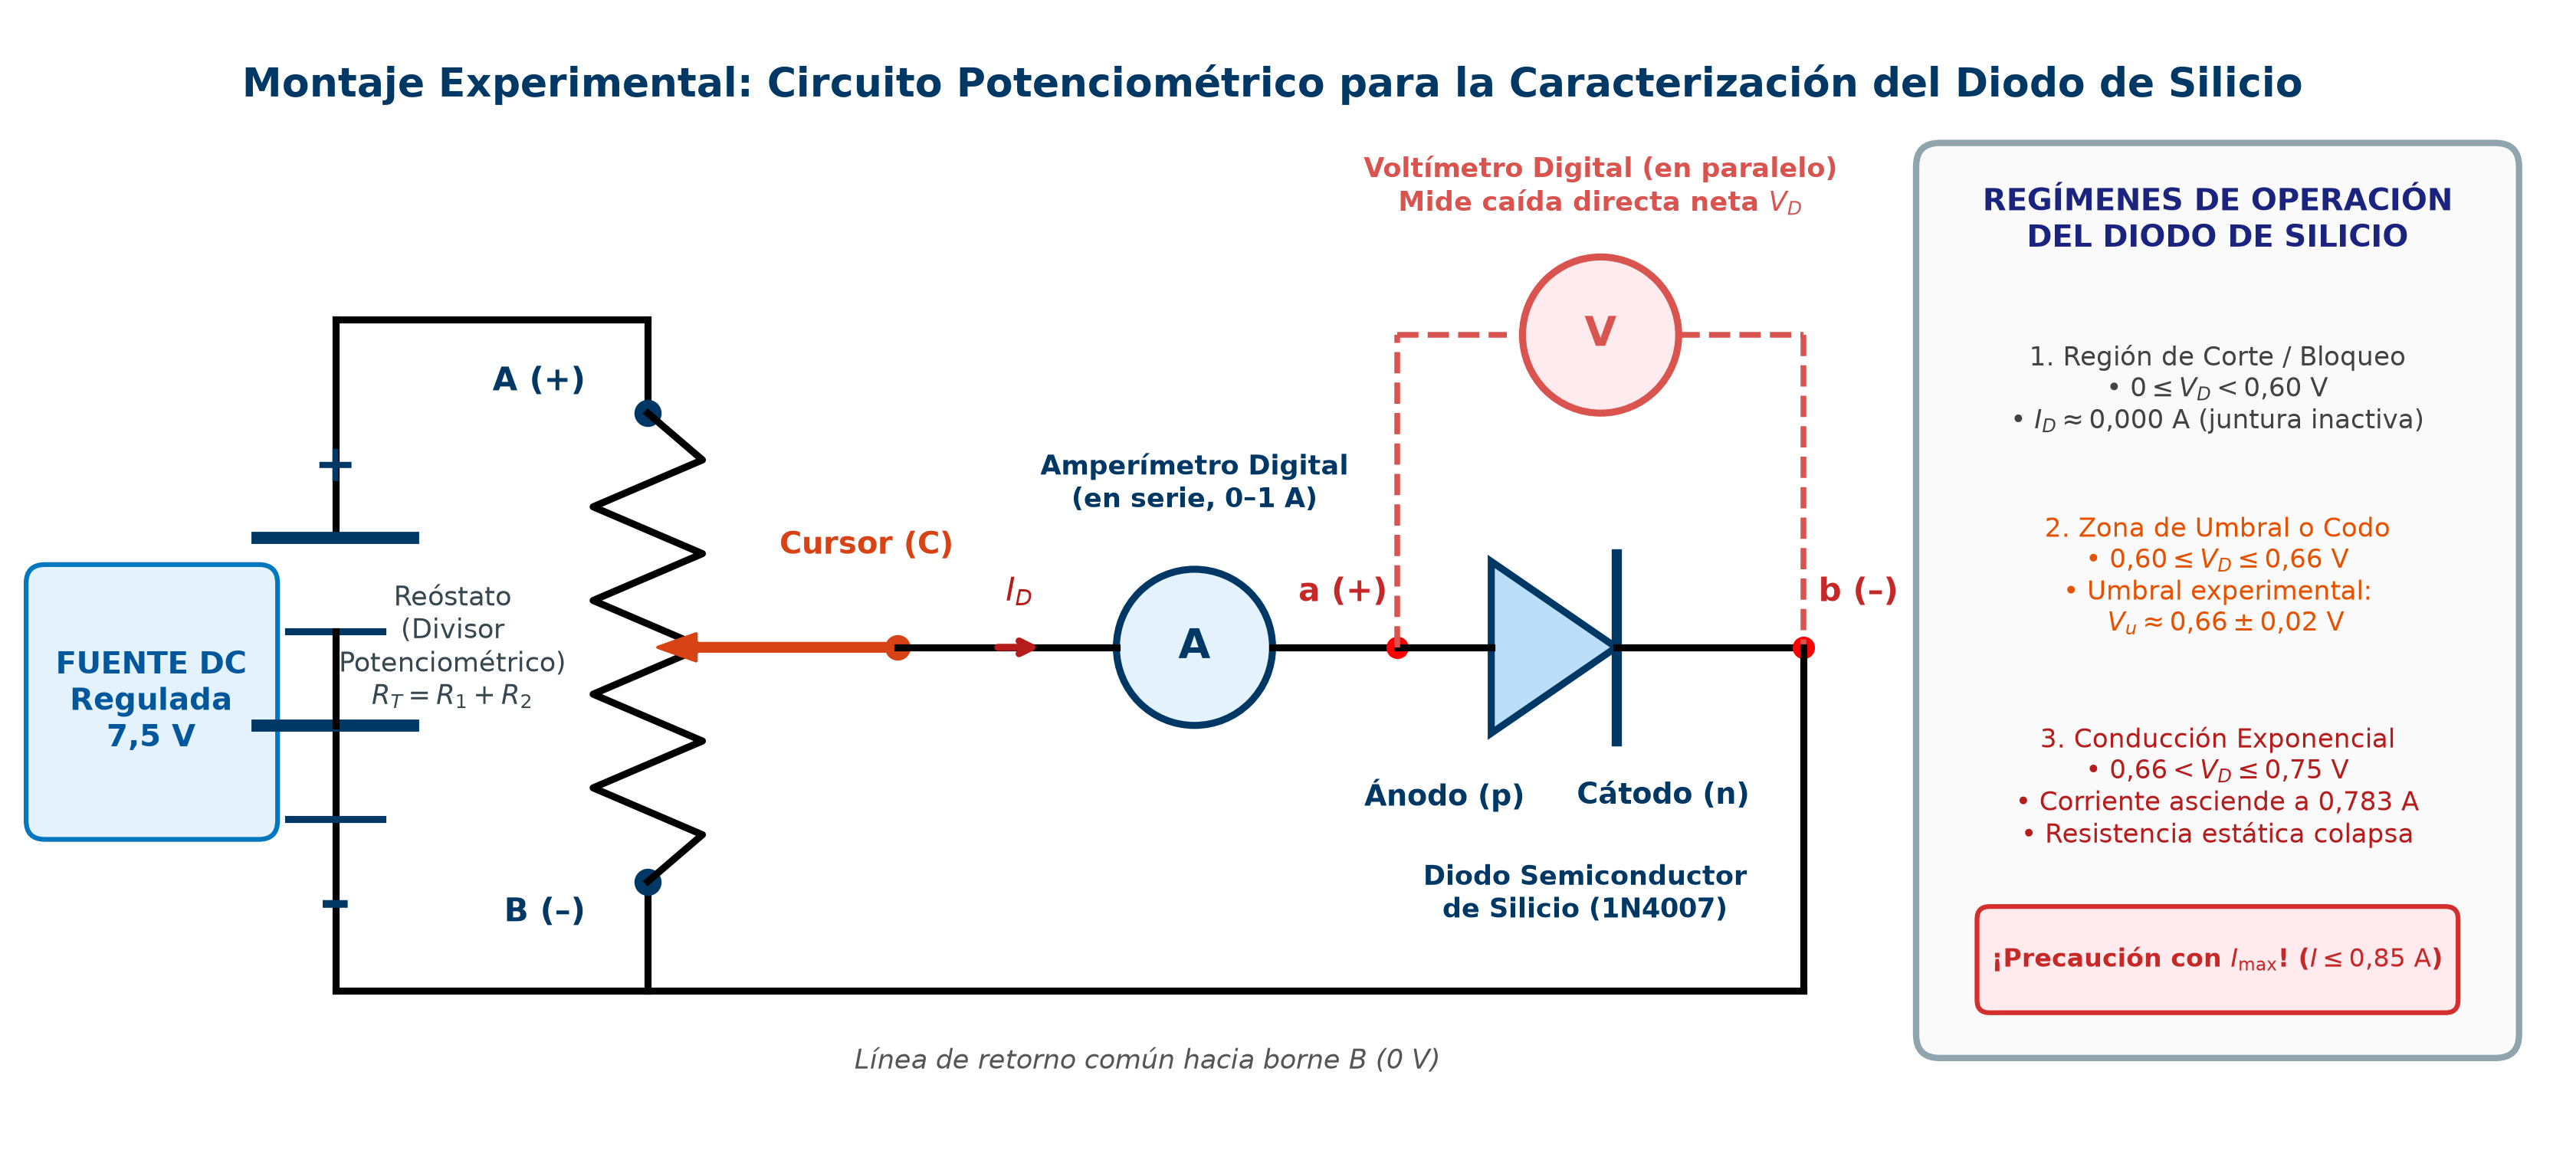
\includegraphics[width=0.96\linewidth]{fig_circuito_diodo_especifico}
    \caption{Diagrama esquemático del circuito experimental implementado para la medición del diodo semiconductor de silicio en polarización directa, detallando el divisor potenciométrico accionado por reóstato, el amperímetro en serie, el voltímetro en derivación paralelo sobre la juntura y las tres regiones características de funcionamiento.}
    \label{fig:circuito_diodo_especifico}
\end{figure}

\textbf{2. Procedimiento experimental seguido paso a paso:}
\begin{enumerate}
    \item \textbf{Identificación de terminales y polaridad:} Previo al conexionado, se inspeccionó físicamente el diodo encapsulado (tipo DO-41, serie 1N400X). Se identificó el \textbf{cátodo} (región $n$) mediante la franja plateada circunferencial en el cuerpo cilíndrico y el \textbf{ánodo} (región $p$) en el extremo opuesto, garantizando que el ánodo se oriente hacia el potencial positivo del cursor.
    
    \item \textbf{Montaje e interconexión del circuito:}
    \begin{itemize}
        \item Se conectó la fuente de alimentación continua estabilizada a $\qty{7,5}{\volt}$ entre los terminales fijos $A$ ($+$) y $B$ ($-$) del reóstato.
        \item Desde el terminal móvil $C$ del cursor se conectó un conductor hacia el borne positivo del amperímetro digital (escala \qtyrange{0}{1}{\ampere}).
        \item El terminal de salida del amperímetro se conectó directamente al ánodo del diodo.
        \item El cátodo del diodo se conectó al terminal común de retorno $B$ del reóstato, cerrando el lazo serie de corriente.
        \item Se instalaron dos sondas de prueba independientes desde el voltímetro digital conectadas en paralelo directo a los bornes ánodo ($a$) y cátodo ($b$) del diodo, para medir la caída directa real $V_D$ libre de caídas parásitas en conductores o en el shunt del amperímetro.
    \end{itemize}
    
    \item \textbf{Ajuste a cero voltios inicial y calibración:} Antes de activar la fuente, se situó el cursor del reóstato en el extremo común $B$, fijando la tensión de salida en $V_{\text{out}} = \qty{0,00}{\volt}$. Se encendió la fuente y se constató que tanto la corriente como el voltaje marcaban cero (\qty{0,00}{\volt}; \qty{0,000}{\ampere}).
    
    \item \textbf{Exploración de la zona de bloqueo o corte (\qtyrange{0,00}{0,60}{\volt}):} Se desplazó suavemente el cursor aumentando la tensión en el diodo. En todo el intervalo inferior a \qty{0,60}{\volt}, la corriente directa permaneció en cero práctico ($I_D \approx \qty{0,000}{\ampere}$), debido a que el potencial aplicado no superaba la barrera de difusión electrostática interna de la juntura $p$-$n$.
    
    \item \textbf{Registro minucioso en la zona de codo y conducción exponencial (\qtyrange{0,60}{0,75}{\volt}):}  
    A partir de los \qty{0,60}{\volt}, se desplazó el cursor con avances micrométricos para registrar pares sincronizados $(V_D, I_D)$:
    \begin{itemize}
        \item \textbf{Punto 2:} \qty{0,61}{\volt} $\longrightarrow$ \qty{0,050}{\ampere} (inicio de la conducción directa).
        \item \textbf{Punto 3:} \qty{0,69}{\volt} $\longrightarrow$ \qty{0,215}{\ampere} (conducción en el codo de la curva).
        \item \textbf{Punto 4:} \qty{0,70}{\volt} $\longrightarrow$ \qty{0,230}{\ampere} (fluctuación instrumental analizada cuantitativamente como outlier estadístico).
        \item \textbf{Puntos 5--8:} Registro secuencial en conducción exponencial a \qty{0,71}{\volt} (\qty{0,411}{\ampere}), \qty{0,72}{\volt} (\qty{0,537}{\ampere}), \qty{0,73}{\volt} (\qty{0,690}{\ampere}) y finalmente a \qty{0,75}{\volt} (\qty{0,783}{\ampere}).
    \end{itemize}
    
    \item \textbf{Retorno seguro y prevención de embalamiento térmico:} Habiendo alcanzado $\qty{0,783}{\ampere}$ (muy próximo al umbral de seguridad de \qty{0,85}{\ampere}), se tomó la lectura inmediata y se retornó con rapidez el cursor a la posición cero, desconectando la fuente para impedir que el calor generado por efecto Joule degradara irreversiblemente la pastilla semiconductora.
\end{enumerate}

%% ------------------------------------------------------------
%%  ANEXO E: Registro Original de Datos y Enunciados
%% ------------------------------------------------------------
\section{Documentación Original de Campo y Registro Facsimilar}
\label{anexo:hoja_datos}

A continuación se incluyen las reproducciones facsimilares de la documentación original generada durante la sesión del Laboratorio \texorpdfstring{N.\textsuperscript{o}\,3}{Nro. 3} (CF2B1, Sección A) el día 01 de octubre de 2026:

\subsection{Enunciado Original del Test \texorpdfstring{N.\textsuperscript{o}\,3}{Nro. 3}}
En la Figura~\ref{fig:test03_enunciado} se reproduce la prueba impresa oficial suministrada por la cátedra de Física III para la evaluación de Curvas Características Voltaje--Corriente.

\begin{figure}[H]
    \centering
    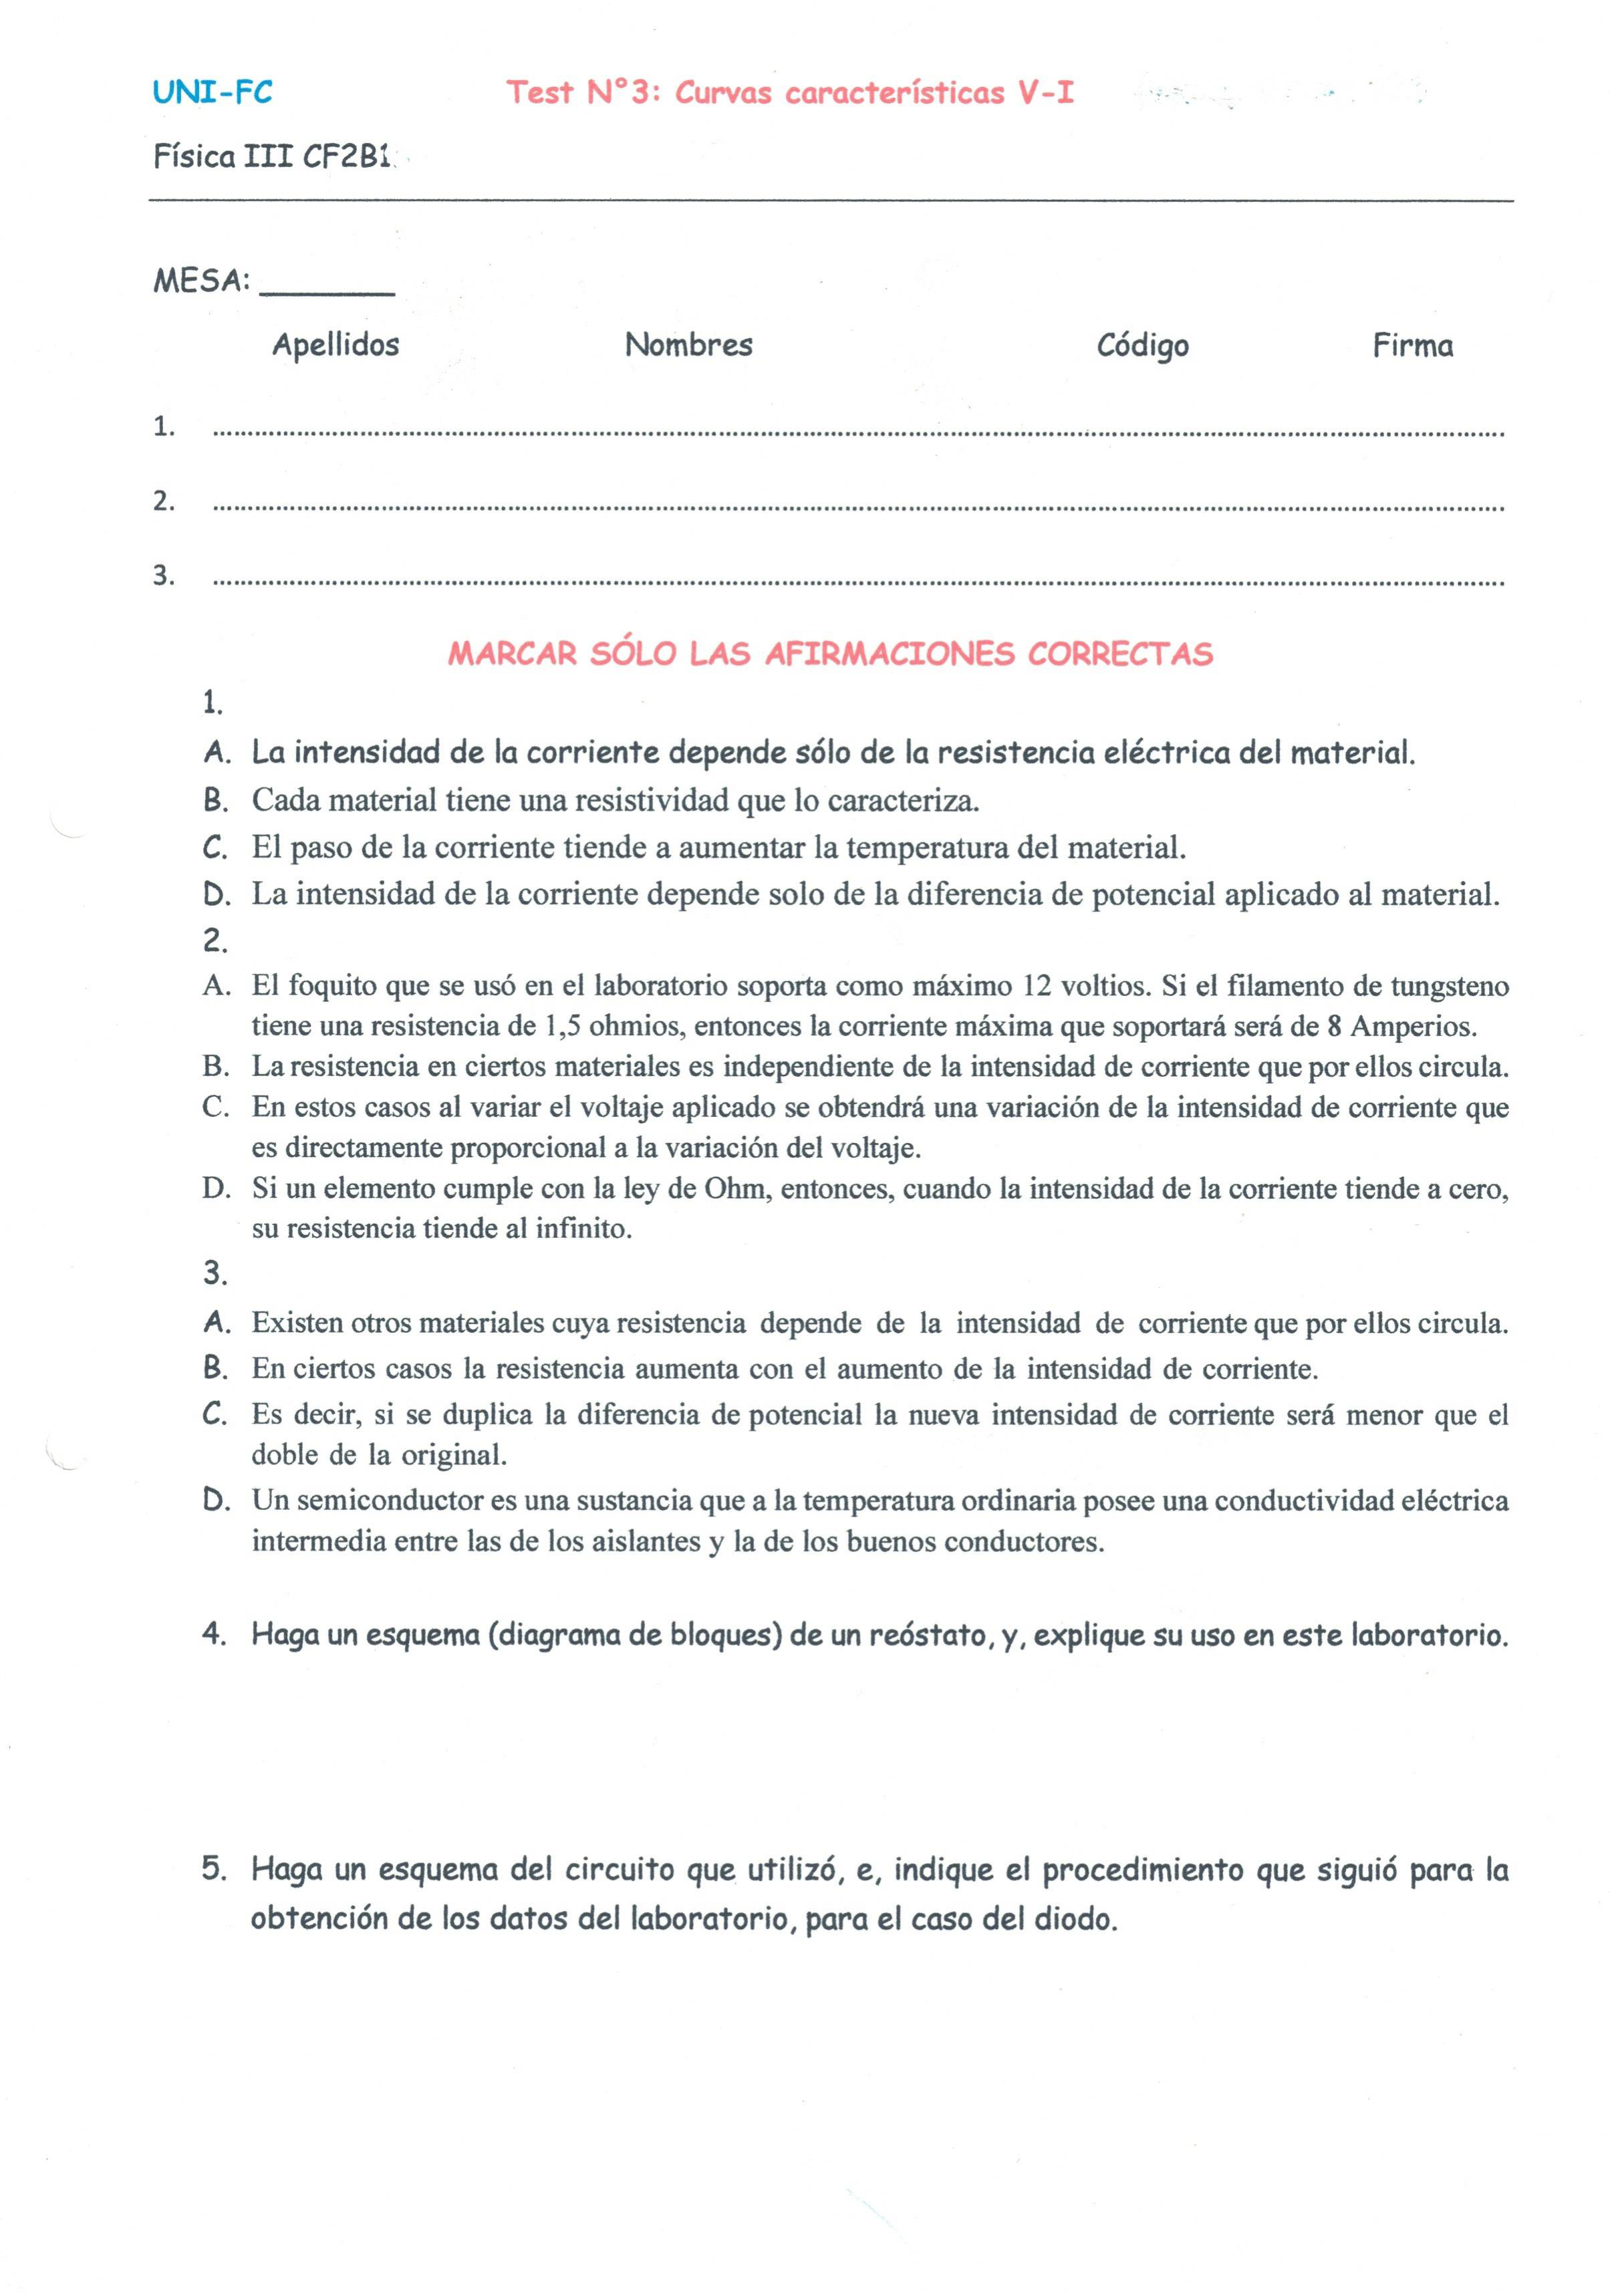
\includegraphics[width=0.88\linewidth]{fig_test03_enunciado}
    \caption{Enunciado facsimilar del Test \texorpdfstring{N.\textsuperscript{o}\,3}{Nro. 3} (Curvas características V--I) de la Facultad de Ciencias de la Universidad Nacional de Ingeniería (Física III CF2B1).}
    \label{fig:test03_enunciado}
\end{figure}

\clearpage
\subsection{Hoja de Datos Experimentales Original Refrendada}
En la Figura~\ref{fig:hoja_datos_original} se reproduce la hoja de toma de datos experimentales original completada in situ en la mesa de trabajo el día 01 de octubre de 2026, suscrita por los integrantes de la mesa (Vera Vivanco Jesús R., Casañe Ramírez Gerald G., Sánchez Feril Piero A.) y debidamente visada por el docente de cátedra.

\begin{figure}[H]
    \centering
    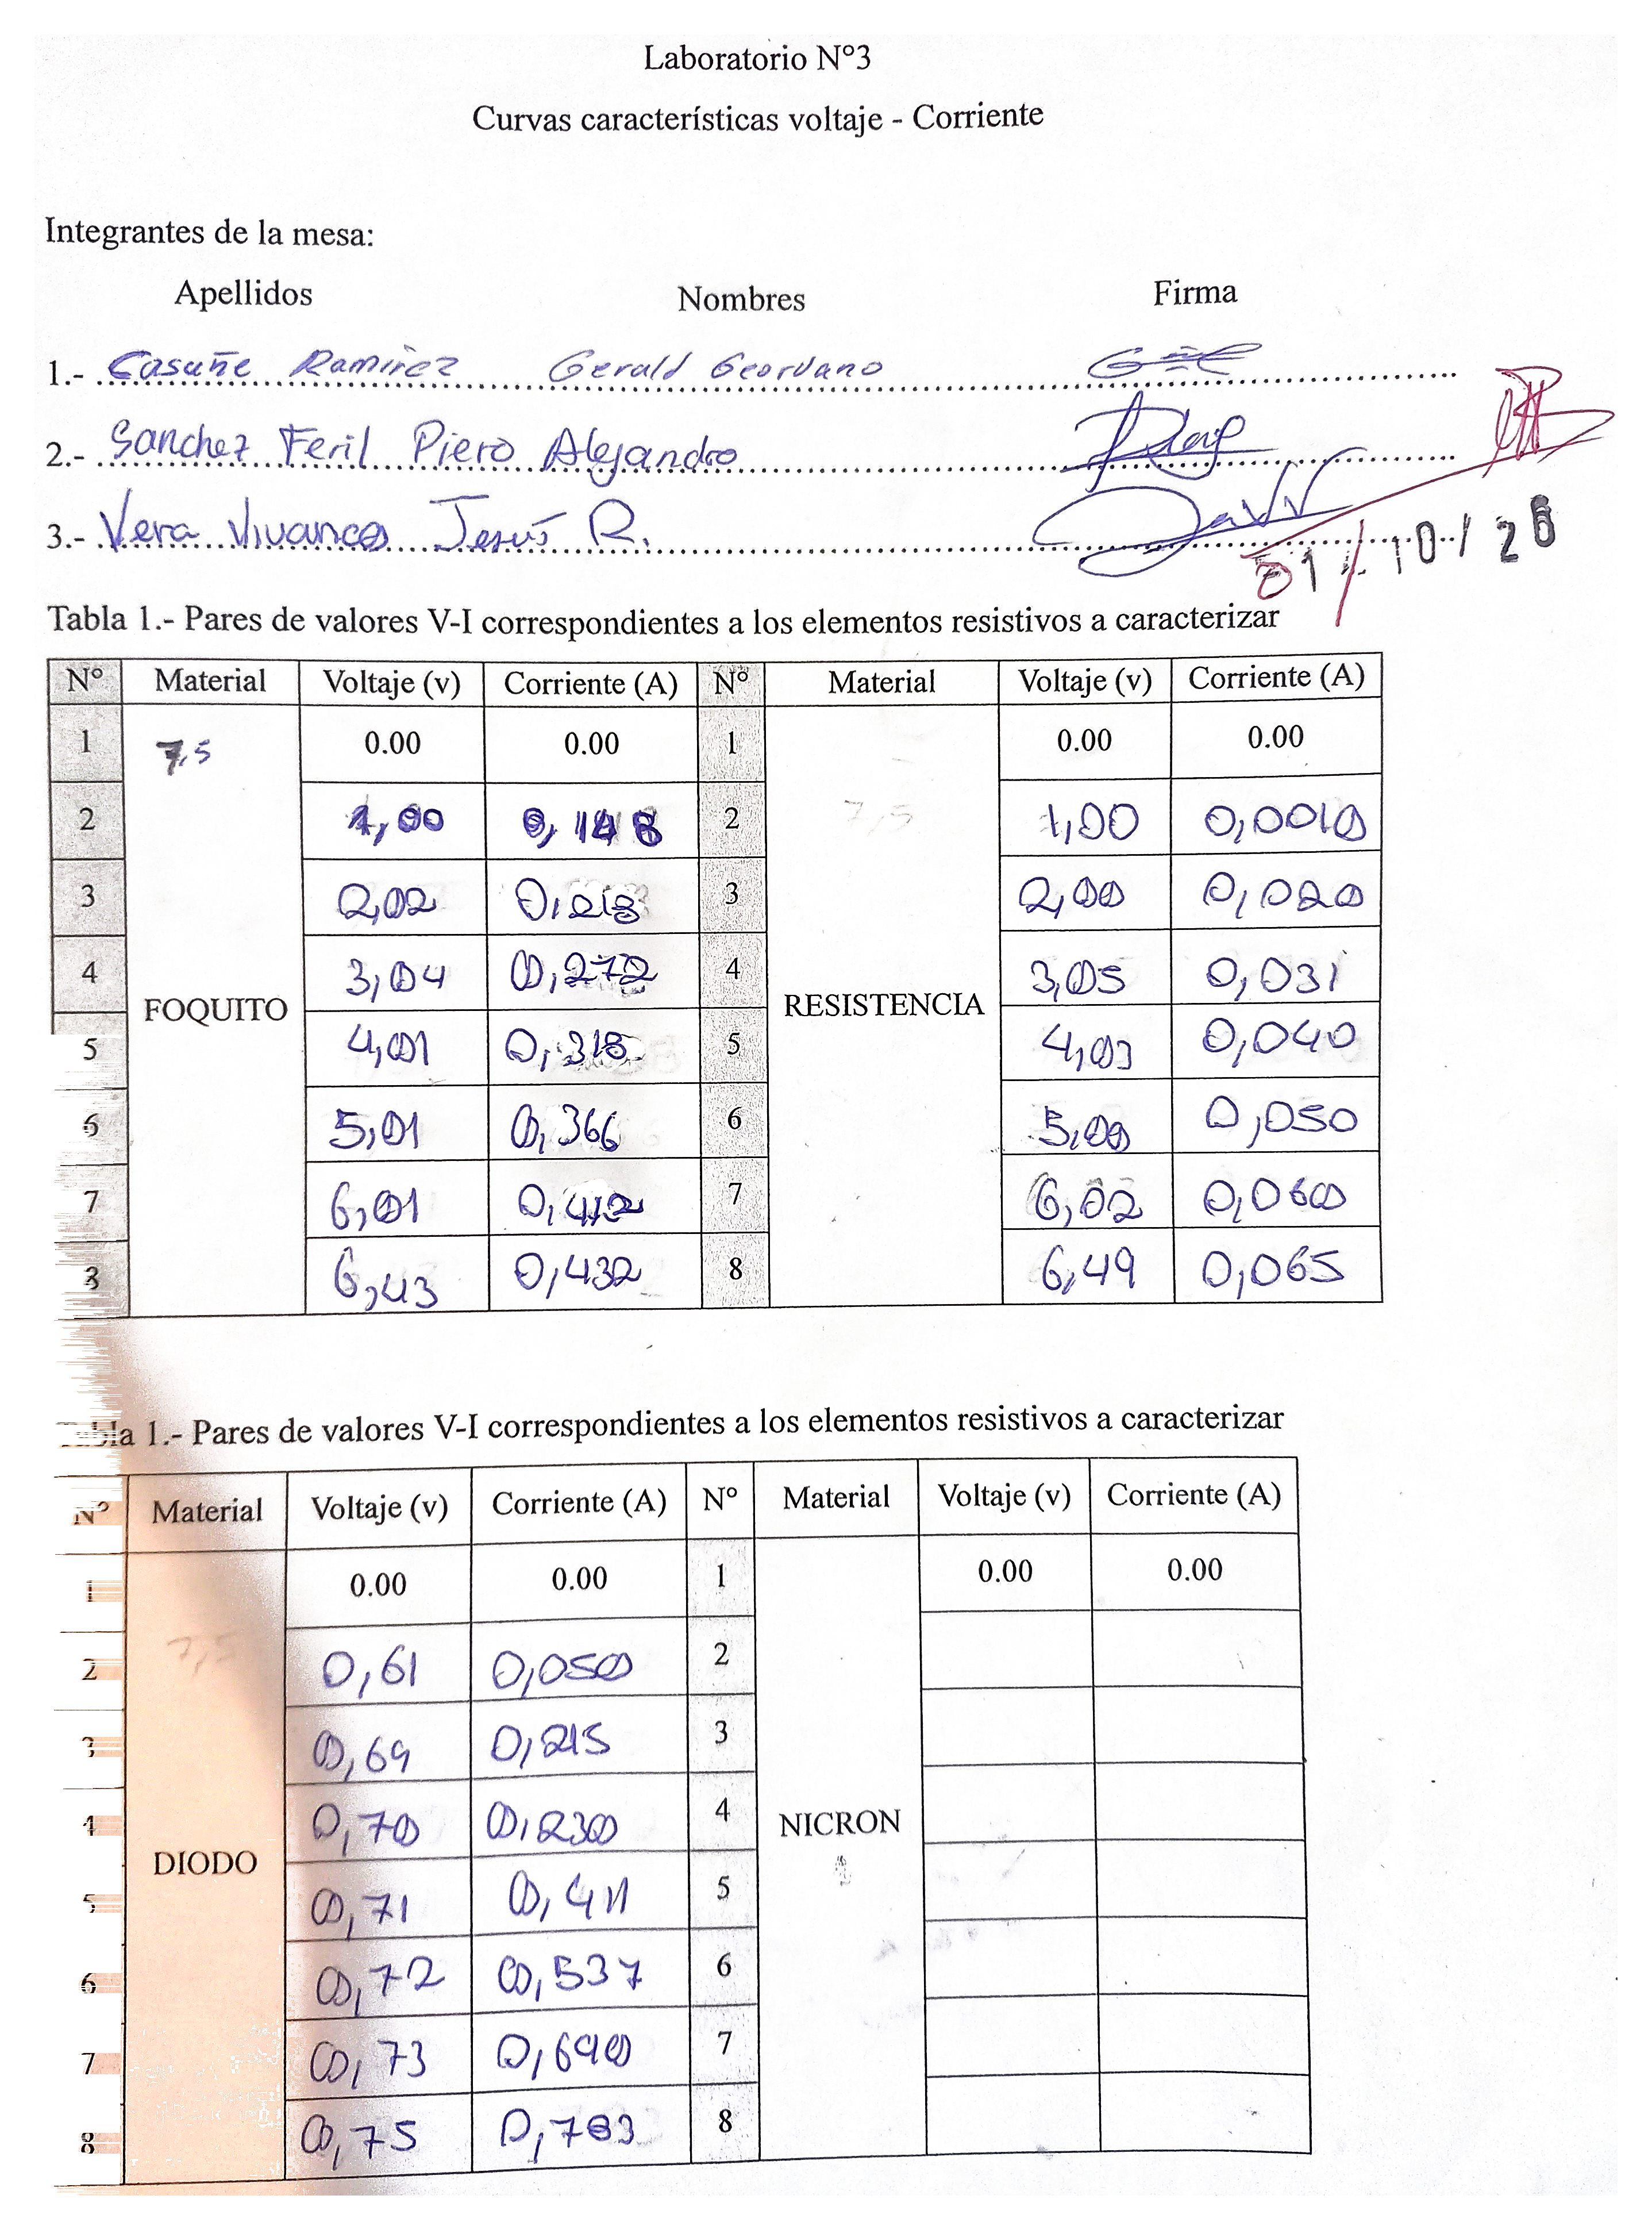
\includegraphics[width=0.88\linewidth]{fig_hoja_datos}
    \caption{Hoja de datos crudos original suscrita en la mesa de trabajo del laboratorio de Física III (CF2B1, Sección A) el 01 de octubre de 2026, con las lecturas directas de voltaje y corriente para el foco de tungsteno, el resistor de carbón y el diodo de silicio, debidamente firmada por los integrantes y visada por la cátedra.}
    \label{fig:hoja_datos_original}
\end{figure}

\end{appendices}
